\documentclass[prb,preprint]{revtex4-1} 

\usepackage{amsmath}
\usepackage{amsfonts}
\usepackage{graphicx}
\usepackage{caption}

\begin{document}

\title{A Measurement of the Electron's Charge to Mass Ratio}

\author{Ryan S. Morshead}
\affiliation{Department of Physics, California State Polytechnic University}

\date{October 8, 2013}

\begin{abstract}
By heating a cathode at one end of a sealed tube to temperatures high enough to ionize particles off its surface, it's possible, to accelerate them through a potential and then expose them to a magnetic field. Once exposed, the stream of accelerated particles -- often called cathode rays -- will be deflected according to Maxwell's equations. By measuring the degree of curvature experienced by the charged particles, voltage of the anode, current through, and radius of, the electromagnet, this paper calculated the charge of the particles in the cathode ray to be $1.73\times10^{11}\pm0.12$ (C/kg). This evaluation of the value for $e/m$ lies within two standard deviations of the accepted value, and a further comparison of the two values yields a percent error of $1.7\%$. Thus this measurement can be said to agree with the accepted value.
\end{abstract}


\maketitle


\section{Introduction}

In October of 1897 Joseph John Thomson published a ground-breaking paper outlining an experiment in which he sought to demonstrate that atoms are actually aggregates of charged particles\cite{jjt}. Prior to this experiment it was generally thought that atoms themselves were the fundamental building blocks of matter. However evidence against this notion began to build when the nature of matter was studied more deeply in the context of large electric fields. It had been observed during these studies that an ionized gas, which was brought into a region between two charged plates, would produce an electric current. The creation of the charged particles was accomplished through the use of a heated cathode which would boil those particles off the surface. It was the unanimous opinion of German physicists that the accelerated particles, also known as cathode rays, were created by some unknown processes in the aether\cite{jjt}. The aether itself was understood to be a homogenous fluid medium; Sir Joseph Larmor had theorized its existence in his book Aether and Matter in 1900 which described the atomic constitution of matter. However Thomson pointed out that no phenomena that had been observed up until that point were analogous to this opinion. Thomson believed that what had been observed suggested that the atoms were being broken down into their charged constituents at the cathode. He eventually went on to prove that the current created by the cathode rays was actually formed by a stream of negatively charged particles moving from the cathode to the anode.

The experiment described in this paper sets out to repeat the results of Thomson's experiment, though with slightly different techniques and equipment.

\section{Experimental Design}

The experiment described here is conducted in the confines of a sealed vacuum tube whose contents are depicted in Figure \ref{datafig}. At one end of the tube a filament is heated to high temperatures by a 6.3 V voltage source. The particles ionized from the surface of the filament, which we assume to have a negative electric charge and mass, are then accelerated through a voltage that's created between the anode and filament. This voltage is denoted here as $V_a$. Once accelerated the particles pass through a slit in the anode and move into the main chamber of the vacuum tube. This cavity, while being surrounded by two Helmholtz Coils, contains a slanted mica screen with Cartesian coordinates printed on it, and horizontal electrodes above and below the mica screen which are kept at the same potential as the anode. The Helmholtz Coils produce a uniform magnetic field ($B$) which is perpendicular to the direction of the particle's velocity. This magnetic field induces a Lorentz force which causes the particles to accelerate in a circular path. The electrodes on the other hand are in place to ensure that there are no electric fields present which could affect the movement of the particles.

	\begin{figure}[h]
		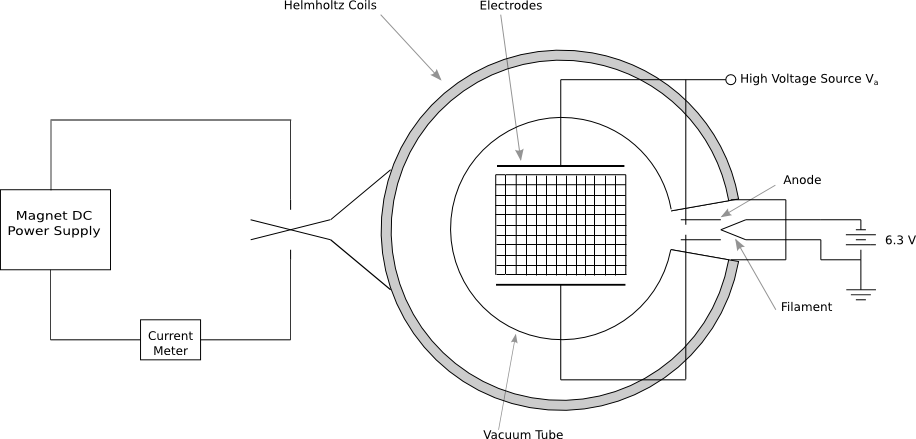
\includegraphics[width=.8\textwidth]{ExpFigure.png}
		\caption{Experimental Arrangement}
		\label{datafig}
	\end{figure}

Under the assumption that the particles are charged, and that due to their velocity in a magnetic field their movements in magnetic field can be explained by Maxwell's equations. Thus the course that the particles take will be circular because their velocity is perpendicular to the magnetic field. As such that path can be modeled by Equation \eqref{eq:eq1} where $r$ is the radius of the circle, and $x_0$ and $y_0$ represent the $x$ and $y$ coordinates of the circle's center respectively.

	\begin{equation}\label{eq:eq1}
		r=\sqrt{\left(x-x_0\right)^2+\left(y-y_0\right)^2}.
	\end{equation}

If we assume the particles initially travel along the x-axis inscribed on the slanted mica screen and begin accelerating to follow their circular path at the moment they exit the slit in the anode, then the center of the particles circular motion will exist directly above the anode. Thus $y_0=r$, and further algebraic manipulation under those assumptions yields Equation \eqref{eq:eq2}.

	\begin{equation}\label{eq:eq2}
		r=\frac{\left(x-x_0\right)^2+y^2}{2y}.
	\end{equation}

Though it's reasonable to assume that the particles only begin to follow their circular trajectory after they leave the slit, as the strong electric field produced by the anode makes any effects from the magnetic field negligible, it's not correct to assume that the particles travel along the x-axis just prior. Thus the experimental procedure which follows moves to account for the inaccuracy of that assumption. This is done by setting the reversing switch attached to the Helmholtz Coils to a neutral position in order to analyze any outside alterations to the particle's trajectory. Then by subtracting these initialized results from the Helmholtz Coil deflection data any extraneous magnetic or electric effects acting on the particles are minimized in the data analysis. Since the minor deflections from the x axis in the absence of the $B$ field are most often curved they may be due to the effects of the earth's magnetic field.

To determine the magnitude of the cathode ray's deflection, the kinetic energy and Lorentz force equations, given by Equation \eqref{eq:eq3} and Equation \eqref{eq:eq4}, are then used in conjunction to find a relationship between $V_a$, $B$, the radius of curvature ($r$), and the ratio of the electric charge (${e}$) to the mass of the particle (${m}$) which can eventually be expressed by Equation \eqref{eq:eq5}.

	\begin{equation}\label{eq:eq3}
		\frac{1}{2}mv^2=eV_a.
	\end{equation}

	\begin{equation}\label{eq:eq4}
		\vec{F}=e\vec{v}\times \vec{B} \implies mv=Ber \implies mv^2=Berv.
	\end{equation}

	\begin{equation}\label{eq:eq5}
		\frac{e}{m}=\frac{2V_a}{B^2r^2}.
	\end{equation}

In the case where relativistic effects should be accounted for, equations \eqref{eq:eq3} and \eqref{eq:eq4} should be modified to account for a relativistic energy and momentum factor of $\gamma$. However, for this experiment, relativistic effects can be said to be negligible as the speed of the particles is significantly smaller than the speed of light. We can show this by taking $V_a$ to be the highest voltage used to calculate $\gamma$ to be about $1.0056$.

\newpage

The strength of the magnetic field present in the vacuum tube, which is created by two parallel Helmholtz Coils with a current $I$ and a diameter $D$ and induces the cathode ray deflection can then be represented by Equation \eqref{eq:eq6}.

	\begin{equation}\label{eq:eq6}
		B=\frac{16\mu_0 N I}{\sqrt{125}D},
	\end{equation}

Where $\mu_0=4\pi\times10^-7 \mbox{ H/m}$ and $N=\mbox{number of turns in the coils}$. With respect to the results produced by this paper a Helmholtz coil with 131 turns and a diameter of $23.25\pm0.1$ cm is used. Now, as is shown by Equation \eqref{eq:eq7}, once all the relevant equations are collected one can create a single expression for the ratio of the particle's charge to its mass.

	\begin{equation}\label{eq:eq7}
		\frac{e}{m}=\frac{2V_a}{\left(\frac{16\mu_0 N I}{\sqrt{125}D}\right)^2\left(r\right)^2}.
	\end{equation}

This is the final relationship which is used in combination with best fit or average values for $r$ and $\delta r$ to derive the measured values for and the error in $e$/$m$ following the necessary measurements of the unknown variables.

\newpage

\section{Results and analysis}

The $(x,y)$ data collected from the mica screen and grid was applied to a least squares optimization of the equation of a circle, thus determining the radius of the circle which best fit the data. The final results for $r$ and $\delta r$ are shown by Figure \ref{LSF:curvature} for a single trial where $V_a$ is equal to 3000 V. The value for ($e$/$m$) was calculated using two different methods; the first being a standard calculation of the mean and the second being a linear curve fit by forming the equation for ($e$/$m$) into the  simple $y=mx+b$ form shown in Equation \eqref{eq:lincurve} where $B^2r^2$ is a function of $2V_a$ and $m$ is the slope and thus equal to $\frac{1}{e/m}$. These two values can be found in Table \ref{e/m by v}. The linear fit value for $e/m$ has an additional graphical representation in Figure \ref{LSF:curvature}.

	\begin{equation}
		\label{eq:lincurve}
		B^2r^2(2V_a) = \frac{2V_a}{m}.
	\end{equation}

	\begin{table}[h]
		\centering
		\caption{Value, and error in, the charge to mass ratio along with other relevant data}
		\begin{ruledtabular}
		\begin{tabular}{c c c c l p{20cm}}
		Trial & $V_a$ (v) & $r\pm \delta r$ (m) & $I(A)$ & $\frac{e}{m}\pm \delta\frac{e}{m}$ (C/kg)\\
		\hline
		1 & $1000\pm$ & $0.291\pm0.004$ & $ 0.35\pm0.01 $ & $1.56\pm0.06\times10^{11}$\\
		2 & $1500\pm$ & $0.278\pm0.004$ & $ 0.42\pm0.01 $ & $1.79\pm0.06\times10^{11}$\\
		3 & $2000\pm$ & $0.286\pm0.004$ & $ 0.49\pm0.01 $ & $1.65\pm0.06\times10^{11}$\\
		4 & $2500\pm$ & $0.286\pm0.004$ & $ 0.54\pm0.01 $ & $1.70\pm0.06\times10^{11}$\\
		5 & $3000\pm$ & $0.292\pm0.004$ & $ 0.59\pm0.01 $ & $1.65\pm0.06\times10^{11}$\\
		\end{tabular}
		\end{ruledtabular}
		\label{e/m by v}
	\end{table}

	\begin{table}[h!]
		\centering
		\caption{Final results for $e/m$ and their comparison with the accepted value}
		\begin{ruledtabular}
		\begin{tabular}{l c c c c p{5cm}}
		Method & $e/m$ & $(e/m)_{accepted}$ & Percent Error (\%)\\
		\hline
		Graphical & $1.73\pm0.12\times10^{11}$ & $1.76\times10^{11}$ & 1.7\\
		Average & $1.67\pm.06\times10^{11}$ & $1.76\times10^{11}$ & 5.11
		\end{tabular}
		\end{ruledtabular}
		\label{final results}
	\end{table}

	\begin{figure}[h!]
		\centering
		\begin{minipage}{.5\textwidth}
			\raggedleft
			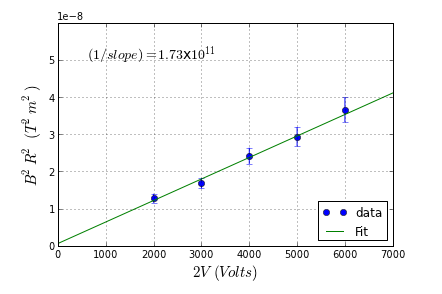
\includegraphics[width= \linewidth]{LinearFinal.png}
			\caption[width = .5\linewidth]{best fit curve to $B^2r^2$ data}
		\end{minipage}%
		\begin{minipage}{.5\textwidth}
			\raggedright
			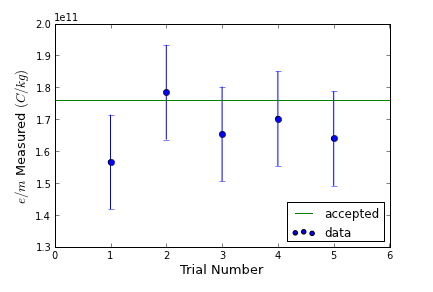
\includegraphics[width=\linewidth]{emFinal.png}
			\caption{Average value of measured $(e/m)$'s}
			
		\end{minipage}
		\label{averages}
	\end{figure}
	
	\begin{figure}[h!]
		\begin{minipage}{.5\textwidth}
			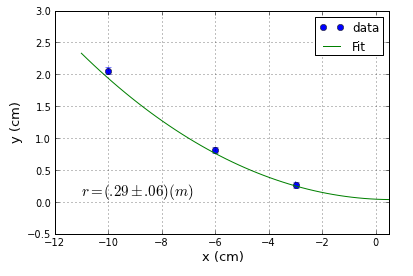
\includegraphics[width=\linewidth]{CircFinal.png}
		\end{minipage}
		\caption{The cathode ray trajectory based on $V_a$ of 3000 V}
		\label{LSF:curvature}
	\end{figure}
	
\newpage

Table \ref{final results} shows that our final result when compared with the accepted value is just under 2\%. This measured value of $1.73\times10^{11}$ C/kg derived from a linear curve fit of the data is a sufficient estimate of the established value for $e/m$ as it lies within two standard deviations of the accepted value. Additionally, the average measurement of $e/m$ managed to yield a value which, though further from the accepted value, still agrees with it when the two are compared.

Five different voltages in the anode were used to measure similar particle trajectories and lessen systematic error. This was done by altering the current through the Helmholtz Coils such that with each new anode voltage the path of the particles would take the same course. Following the collection of the radii for the Helmholtz Coils and initialized trajectory data, six data points on the mica screen, in addition to the corresponding $I$ value, were collected for each anode voltage; three for each direction on the reversing switch. The result being that data was collected on two different, but near perfect mirror trajectories, thus minimizing systematic error even further. 

\section{Conclusion}

The purpose of this experiment was to, with some degree of accuracy, measure the mass to charge ratio of electrons and thus replicate the pivotal results which Joseph John Thomson found in 1897. The values for $e/m$ which this experiment reports agree with the accepted value.

\newpage

\begin{acknowledgements}
Thank you to Jennifer, all my physics teachers, past and present, and the all too glorious \textit{Google}, for help and encouragement through this terribly arduous process.
\end{acknowledgements}

\begin{thebibliography}{99}

\bibitem{jjt} J. J. Thomson, (1856-1940) Philosophical Magazine, \textbf{44}, 293 (1897).

\bibitem{aether} Joseph Larmor, ``Aether and Matter'', Cambridge University Press, 1900, Chapters X-XI (pp. 161-193)

\end{thebibliography}

\end{document}